\section{Day 5: Trees (Sept 15, 2025)}

\begin{definition}[Binary Search Tree Property]
For each node $x$ in the binary tree,
\begin{itemize}
\item If $y$ is in $x$'s left subtree, $y.key \leq x.key$ 
\item If $z$ is in $x$'s right subtree, $z.key \geq x.key$
\end{itemize}
\end{definition}

A BST has $\Theta(n)$ insert, delete, and search operations. The main issue is that the entire tree can behave like a linkedlist, where we do not make use of the other child field. We aim to solve this by using AVL trees, which have the aforementioned operations but in $\log_2 n$ time. 

Recall that \textsc{Delete}($T$, $z$) where $z$ is a pointer to the node to be deleted, can be achieved as follows:
\begin{itemize}
\item If $z$ is a leaf, replace the reference with \textsc{Nil}
\item If $z$ has 1 child, replace the reference to $z$ with its child
\item If $z$ has 2 children, replace $z.key$ with its successor key and delete the successor node. 
\end{itemize}
\noindent The successor of $z$ is the node you get by going right once and left repeatedly.

\begin{definition}[Ideally Height-Balanced]
A binary tree is \textit{ideally height-balanced} if every leaf has depth $h$ or $h-1$, and every node at depth less than $h - 1$ has 2 children. 
\end{definition}
Reminiscent of a balanced binary tree, except the last row need not be filled in left to right order. An ideally height balanced tree with $n$ nodes has height $\lfloor \log_2 n \rfloor$ just like a balanced binary tree of the same size.

Creating an ideally balanced binary tree is difficult to do in logarithm time, unsure if there are any lower bound results on this. The difficulty of this problem motivates the following definition, where we loosen the idea of an ideally height-balanced tree

\begin{definition}[Height-Balanced]
A binary tree is \textit{height-balanced} if for every node, the heights of its left and right subtrees differ by at most 1.
\end{definition}

\begin{definition}[Balance Factor]
    $BF(x) = height(x_R) - height(x_L)$. Let $y$ be a node with 1 child. Define $BF(\textsc{Nil}) = -1$, $BF(y) = 0$.
\end{definition}

We call a height-balanced BST an \textbf{AVL tree}. To be an AVL tree, for all nodes $x$, $BF(x) \in \{ -1, 0, 1 \}$.

\begin{simplethm}
    The height of an AVL tree with $n$ nodes is $O(\log_2 n)$ .
\end{simplethm}
\begin{proof}
    Let $M(h)$ denote the minimum number of nodes in an AVL tree with height $h$. By property of AVL tree, we have that $M(0) = 1, M(1) = 2, M(h) = 1 + M(h - 1) + M(h - 2) = F_{h + 3} + 1$. From number theory facts (MAT315), $F_n > \frac{\phi^h}{\sqrt{5}} - 1$, where $\phi = \frac{1 + \sqrt{5}}{2}$. $n \geq M(h) > \frac{\phi^{h+3}}{\sqrt{5}} - 2$. Then we get
    \[
    h < 1.44 \log_2 (n + 1) 
    \]
\end{proof}

For the insert position, suppose that the insert has successfully occurred. Only the balance factors of nodes that have $x$ in their subtree get updated. Some may end up with a more than 2 balance factor, which needs addressing.

\subsection{Tree Rotations}

There are 4 types of tree rotations, being the single left and right rotation, and the double left-right and right-left rotation. After \textsc{Insert}($x$), one of $T_1$, $T_2$, or $T_3$ will receive the additional node. In below figure, $T_3$ for the left side tree and $T_1$ for the right side tree getting $x$ is not a concern, as in this case all of $T_1, T_2, T_3$ are of height $h$. 

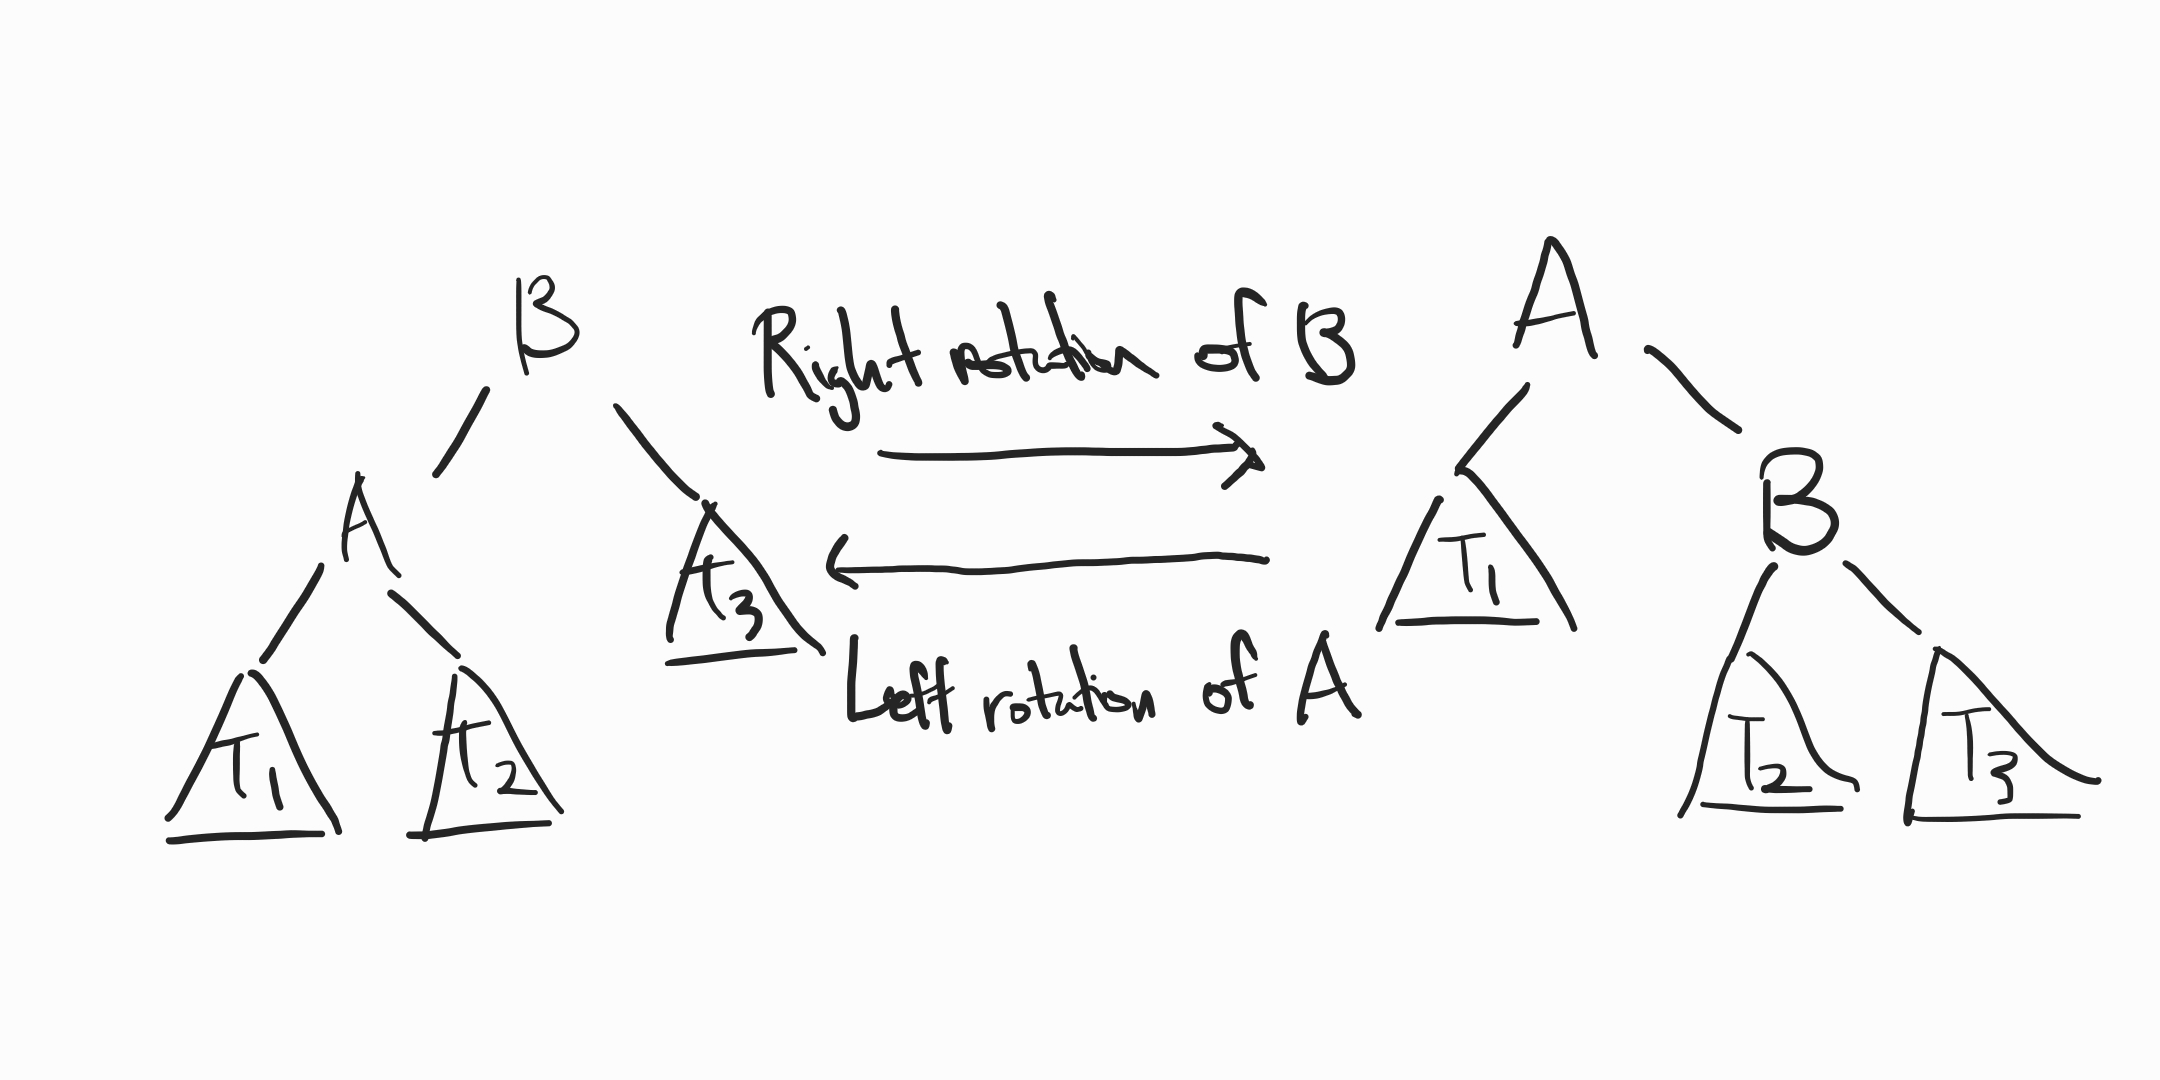
\includegraphics{csc265/figures/avlleftandrightrotation.jpg}

You would use the single right rotation on the left-side figure when $x$  is added to $T_1$, where $A$ has a negative balance factor. We use the single left rotation on the right-side figure when the violation is in $T_3$, where $B$ has a positive balance factor.

This leaves the case where $A$ has a positive balance factor in the left figure ($T_2$ has bigger height than $T_1$), and the case where $B$ has a negative balance factor ($T_2$ has bigger height than $T_3$). Note that the two cases are mirror images of each other, where we simply flip the signs of the balance factor:

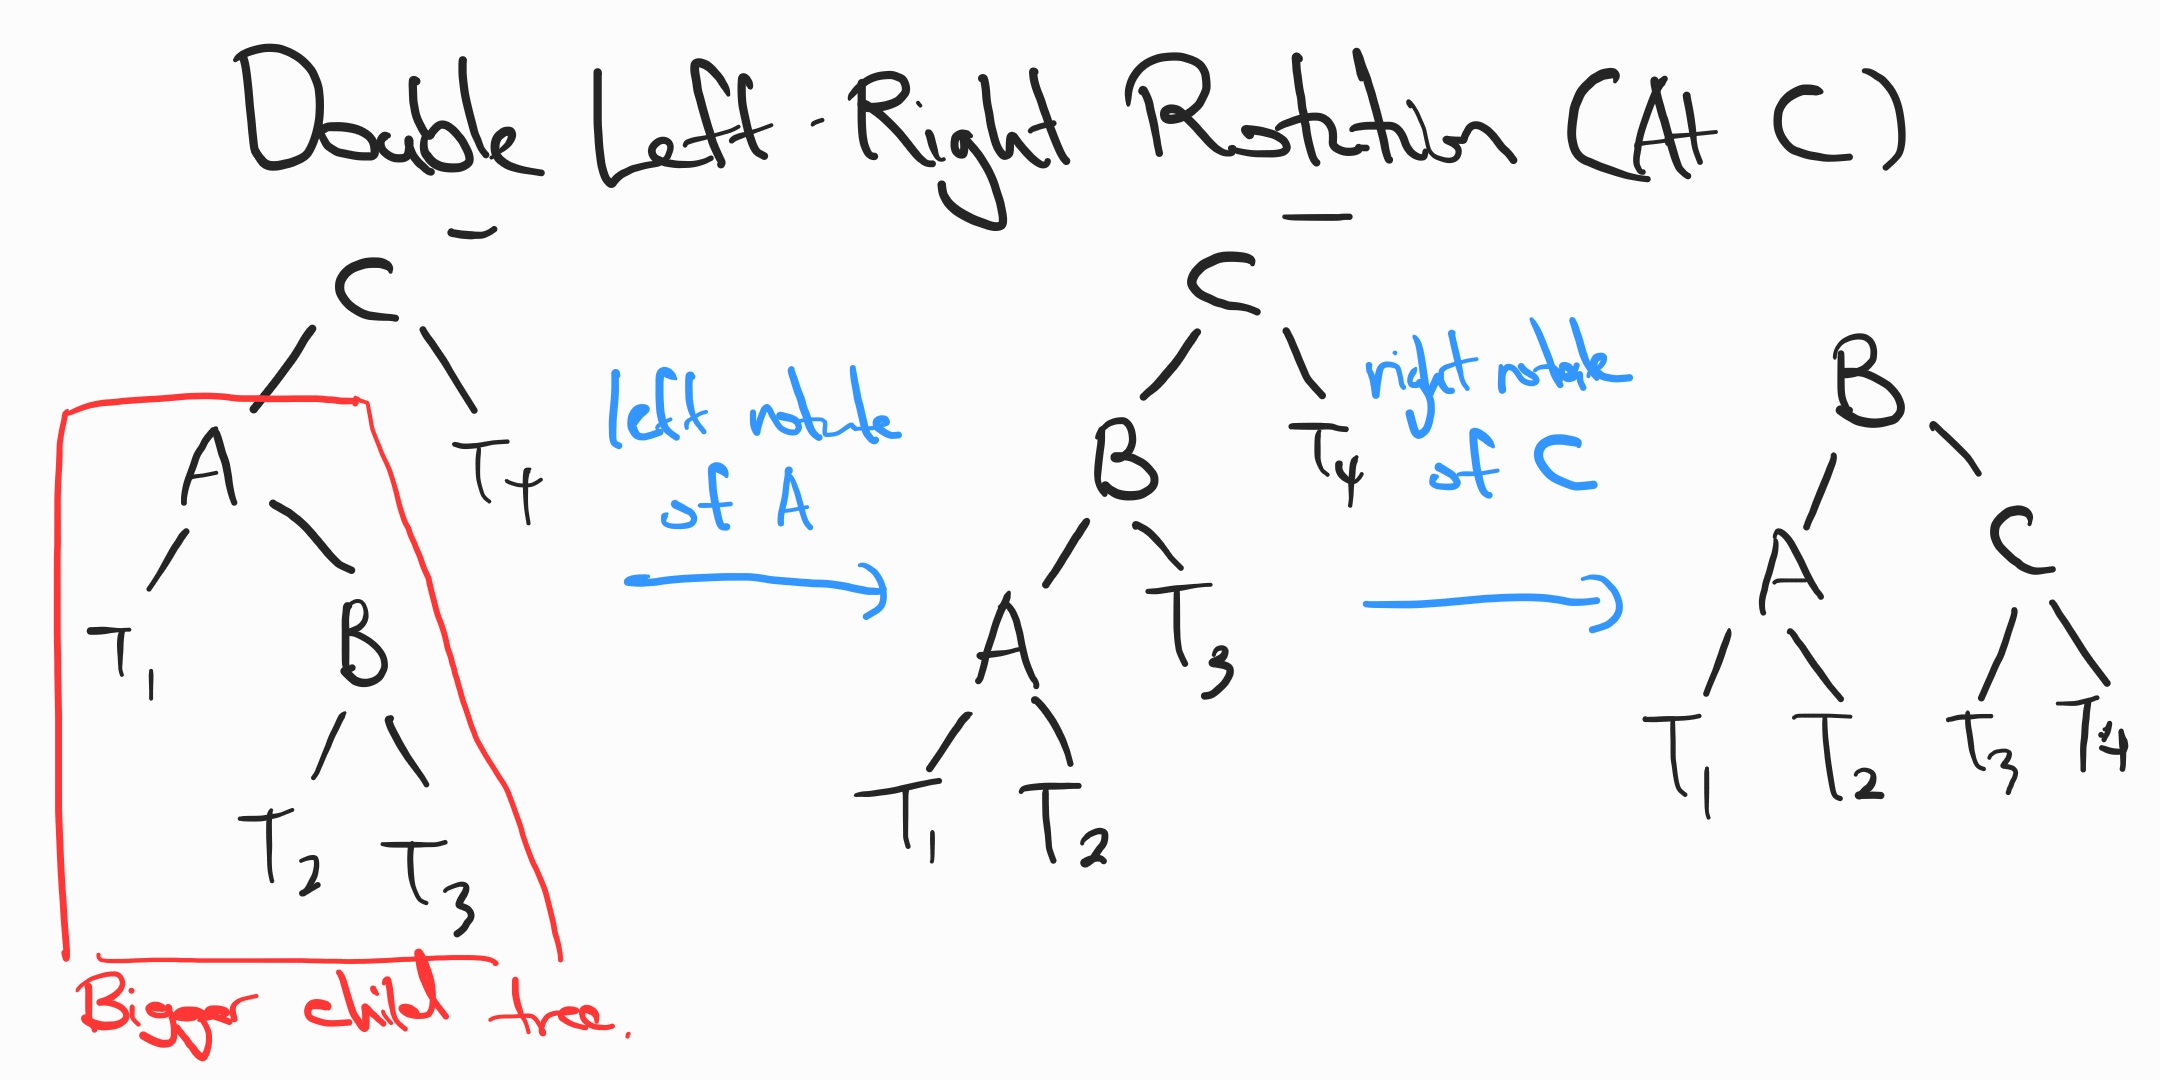
\includegraphics{csc265/figures/avldoubleleftrightrotation.jpg}

In this figure note that $A$ has a positive balance factor, C has a unacceptably negative balance factor, which we then handle using a double left right rotation. In the mirror image, $A$ will have a negative balance factor, $C$ will have an unacceptably positive balance factor, where we use a double right left rotation. 

\begin{remark}
If you see this on the midterm and you're not sure which one you should do, just do all 4 rotations and eventually 1 will work.
\end{remark}

\noindent To insert on an AVL tree, we perform steps as follows:
\begin{itemize}
\item Insert new node $x$ following standard BST insert
\item From inserted node up to root, update balance factor and do rotations to fix the imbalance
\end{itemize}

\begin{claim}
We only need to do at most one  single or double rotation for \textsc{Insert}.
\end{claim}
You would prove this by doing a ton of cases. Also start assignment 2 early! It's hard - Jeremy Ko.
